%!TEX program = xelatex
%!BIB program = bibtex

\documentclass[en,black,12pt,normal]{elegantnote}
\usepackage{float}
\usepackage{hyperref}

\newcommand{\upcite}[1]{\textsuperscript{\textsuperscript{\cite{#1}}}}

\title{Bioinformatics Practical 1\\\small{Navigating through NCBI 2021.3}}
\author{WenYuan Jiang\\ID: 1951510}
\institute{School of Life Science, Tongji University}
%\version{1.00}
\date{March 13, 2021}

\begin{document}

\maketitle


\section{Question:}
\textit{List some databases that stores scientific literatures. List some bioinformatics related journals (including database/server related journals).}

\subsection*{Solution:}

Some scientific literature databases are listed below.\upcite{wiki:List_of_academic_databases_and_search_engines}
Note that some of the databases are not limited to the life science field.
\begin{itemize}
    \item Google Scholar\upcite{gusenbauer2019google}:
        \subitem The biggest academic database \& search engine (over 390 million records, unofficial estimate).
    \item PubMed\upcite{fiorini2017cutting}:
        \subitem A database primarily of references and abstracts on life sciences and biomedical topics. Includes MEDLINE, PubMed Central, and Bookshelf.
    \item PubMed Central\upcite{roberts2001pubmed}:
        \subitem Free full-text archive of publications and preprints.
    \item Europe PMC\upcite{europe2015europe}
        \subitem Abstracts \& full text (6.5 million) biomedical and life sciences articles (Dec 2020). Includes text mining tools and links to external molecular and medical data sets.
    \item Web of Science\upcite{mongeon2016journal}
        \subitem A multidisciplinary scientific literature database. Includes other products, such as Social Science Citation Index, Science Citation Index, Biological Abstracts \& The Zoological Record.
    \item Science Direct
        \subitem Content from more than 4,000 academic journals and 30,000 e-books in the field of science and medicine.
    \item CNKI\upcite{yu2005cnki}
        \subitem A comprehensive China Integrated Knowledge Resources System, including journals, doctoral dissertations, masters' theses, proceedings, newspapers, yearbooks, statistical yearbooks, ebooks, patents, standards and so on.
    \item arXiv\upcite{wiki:ArXiv}
        \subitem A multidisciplinary open-access repository of electronic preprints (known as e-prints) approved for posting after moderation, but not peer review.
\end{itemize}
More databases can be found using search engines like Google or Bing, if proper key words like \texttt{literature databases} are provided.

Some bioinformatics related journals are shown below.\upcite{wiki:List_of_bioinformatics_journals}
\begin{itemize}
    \item \textit{Nucleic Acids Research}, Oxford University Press, IF=11.501 (2019)
    \item \textit{Bioinformatics}, Oxford University Press, IF=5.610 (2019)
    \item \textit{BMC Bioinformatics}, 	BioMed Central, IF=3.242 (2019)
    \item \textit{Briefings in Bioinformatics}, Oxford University Press, IF=8.990 (2019)
    \item \textit{Cancer Informatics}, SAGE Publications, IF=1.21 (2018)
    \item \textit{IEEE/ACM Transactions on Computational Biology and Bioinformatics}, Institute of Electrical and Electronics Engineers and Association for Computing Machinery, IF=3.015 (2019)
    \item \textit{Database: The Journal of Biological Databases and Curation}, Oxford University Press, IF=2.593 (2019)
    \item \textit{Computational Biology and Chemistry}, Elsevier, IF=1.850 (2019)
    \item \textit{PLOS Computational Biology}, Public Library of Science, IF=4.428 (2018)
\end{itemize}

\section{Question:}
\textit{Perform a simple text query for articles on 2019 novel coronary infection pneumonia in pubmed, please paste your keywords and the number of hits.}

\subsection*{Solution:}
The keywords in the query are \texttt{((2019 novel coronavirus) AND (infection)) AND (pneumonia)}, and the number of hits is 53,296.

\section{Question:}
\textit{Many papers were analyzed by bioinformatics in above results, please briefly introduce one of them.}

\subsection*{Solution:}
One of the papers in above results is titled \textit{Genomic characterization of the 2019 novel human-pathogenic coronavirus isolated from a patient with atypical pneumonia after visiting Wuhan},
authored by Chan te al.\upcite{chan2020genomic}

By analyzing the 2019 novel coronavirus genome, the paper provided us with the Genome organization of 2019-nCoV. Phylogenetic relationship among 2019-nCoV and other βCoVs is also given in the paper
by comparing the 2019-nCoV HKU-SZ-005b sample with other related strains collected from human or mammals. Techniques involved are multiple alignment (CLUSTAL 2.1), 
phylogenetic tree construction by the neighbour joining method (MEGA X), PSI-blast-based secondary structure PREDiction (PSIPRED), 
prediction of protein secondary structure (neural networking),
prediction of transmembrane domains (TMHMM 2.0),
secondary structure prediction in the 5′-untranslated region (UTR) and 3′-UTR (RNAfold WebServer).

\section{Question:}
\textit{From your search results, are there any articles that appear to be irrelevant (these are known as \textbf{false positives}, as opposed to \textbf{true positives} which refer to hits that are relevant) to your search term? How would you make your search term more specific, with less \textbf{false positives}?}

\subsection*{Solution:}
Irrelevant hits do exist in the results. An example of false positives is the \textit{Liver injury during highly pathogenic human coronavirus infections}\upcite{xu2020liver} by Xu et al.

To make the search term more specific, more filters could be added, and some unspecific keywords like \texttt{infection} can be removed.

After removing \texttt{infection} and adding \texttt{NOT (liver)}, we get 52,733 results, which are more desirable.

\section{Question:}
\textit{How often is the NCBI Nucleotide database updated? Draw a plot about the records in GeneBank, the Y-axis is the number of bases and the number of sequences from the beginning to the present of GenBank and WGS respectively, the X-axis is the year. Write your comments on this figure.}

\subsection*{Solution:}
The Nucleotide database is updated every day. Records from the International Collaboration databases DDBJ and EMBL are added on a nightly build. 

The required figure is shown below.
\begin{figure}[H]
    \centering
    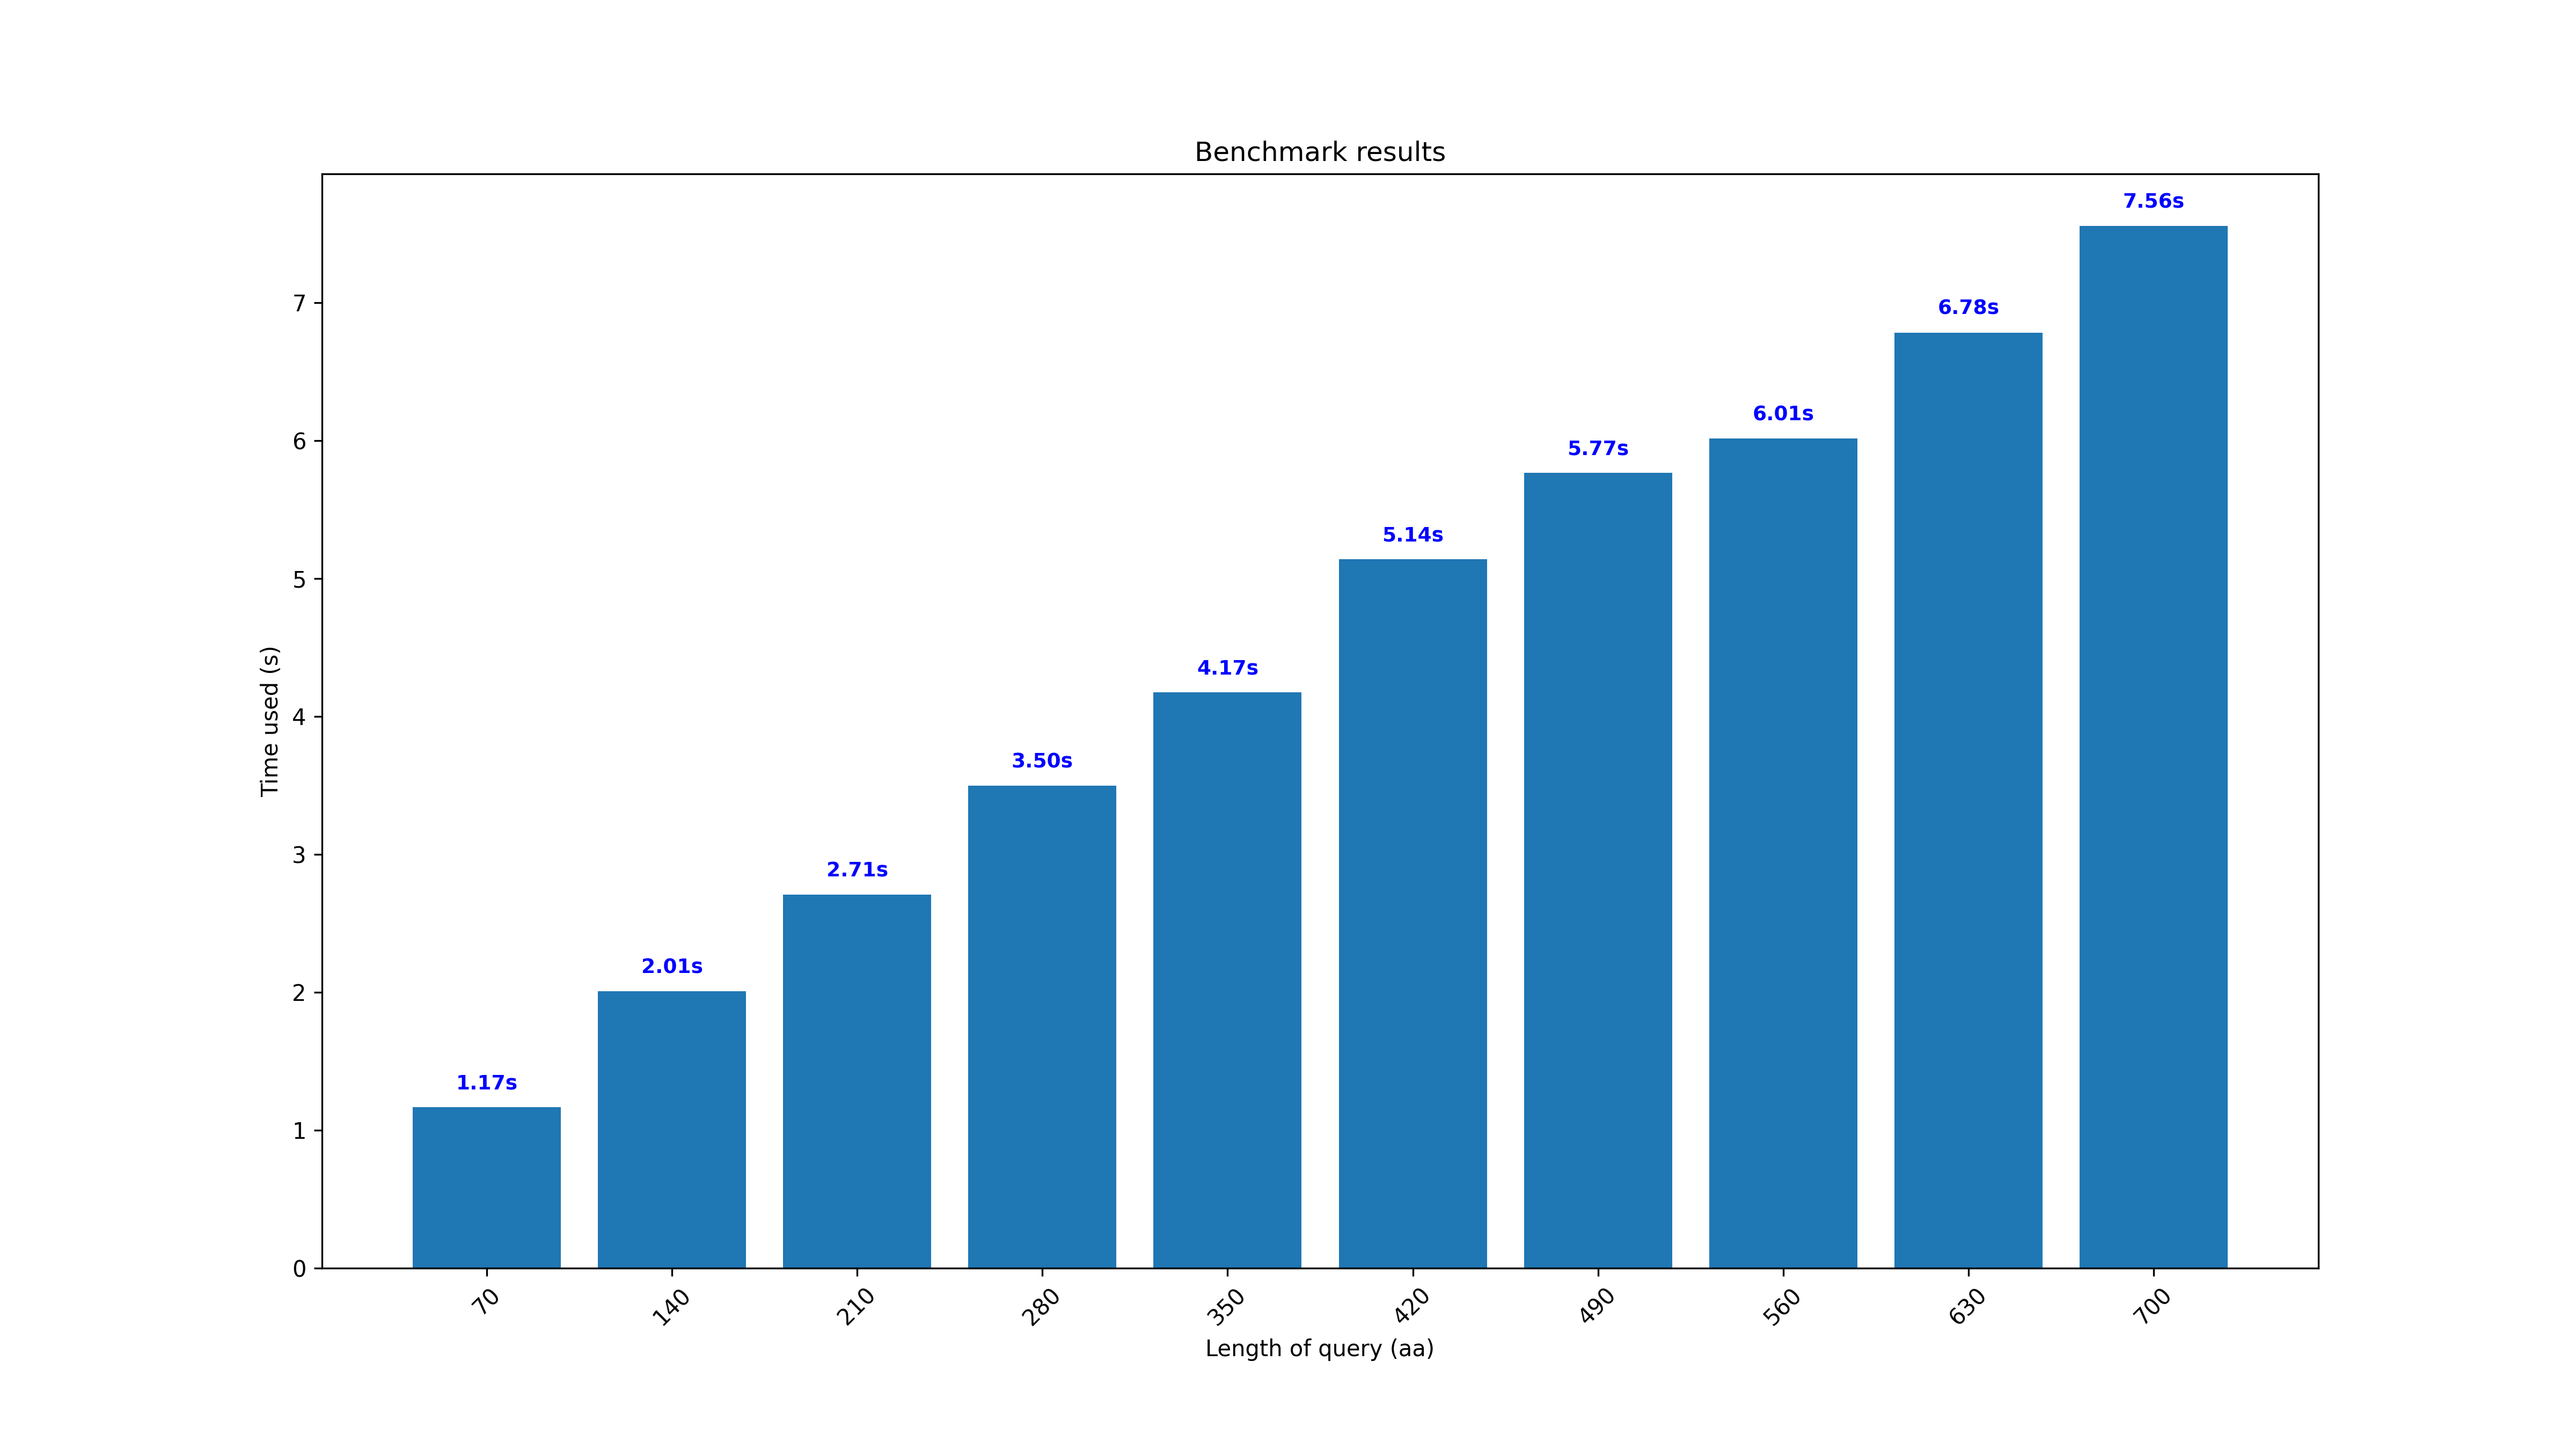
\includegraphics[width=1\textwidth]{Fig01}
    \caption{}
    \label{F-01}
\end{figure}

From the plot, it can be seen that the volumn of data in GenBank and WGS is growing \textbf{exponentially}, 
which is not surprising considering the advanced sequencing technology.
With massive amount of sequencing data, it brings us a challenge of how to interprete these data,
since data without proper interpretation has little value.

\section{Question:}
\textit{Search 2019-ncov in nucleotide database, and select an entry to view the full record:}
\begin{itemize}
    \item \textit{What is the accession number of the record?}
    \item \textit{What is the version number of the record?}
    \item \textit{Which organism is this sequence from?}
    \item \textit{What is the taxonomic lineage for this organism?}
    \item \textit{What is the taxonomy identifier (Taxon ID)?}
    \item \textit{What is name of the nucleotide sequence?}
    \item \textit{Notice the specific features of the FASTA format. Describe them.}
    \item \textit{Write down the Gene Id and name of this sequence.}
    \item \textit{Write down one of the products of this sequence and its protein\_id. Which database does this link to?}
    \item \textit{How many amino acids (aa) constitute this protein?}
\end{itemize}

\subsection*{Solution:}
\begin{itemize}
    \item \textit{What is the accession number of the record?}
    \subitem MN988668
    \item \textit{What is the version number of the record?}
    \subitem MN988668.1
    \item \textit{Which organism is this sequence from?}
    \subitem Severe acute respiratory syndrome coronavirus 2
    \item \textit{What is the taxonomic lineage for this organism?}
    \subitem Viruses; Riboviria; Orthornavirae; Pisuviricota; Pisoniviricetes;
    \subitem Nidovirales; Cornidovirineae; Coronaviridae; Orthocoronavirinae;
    \subitem Betacoronavirus; Sarbecovirus.
    \item \textit{What is the taxonomy identifier (Taxon ID)?}
    \subitem Taxonomy ID: 2697049
    \item \textit{What is name of the nucleotide sequence?}
    \subitem Severe acute respiratory syndrome coronavirus 2 isolate 2019-nCoV WHU01, complete genome
    \item \textit{Notice the specific features of the FASTA format. Describe them.}
    \subitem The description line (defline) or header/identifier line, which begins with '>', gives a name and/or a unique identifier for the sequence, and may also contain additional information.
    \subitem Following the header line, the actual sequence is represented. Sequences may be protein sequences or nucleic acid sequences, and they can contain gaps or alignment characters. 
    Sequences are expected to be represented in the standard IUB/IUPAC amino acid and nucleic acid codes, with these exceptions: lower-case letters are accepted and are mapped into upper-case; a single hyphen or dash can be used to represent a gap character; and in amino acid sequences, U and * are acceptable letters.
    \subitem A multiple sequence FASTA format would be obtained by concatenating several single sequence FASTA files in a common file (also known as multi-FASTA format). \upcite{wiki:FASTA_format}
    \item \textit{Write down the Gene Id and name of this sequence.}
    \subitem GI: 800455117
    \subitem Name: Severe acute respiratory syndrome coronavirus 2 isolate 2019-nCoV WHU01, complete genome
    \item \textit{Write down one of the products of this sequence and its protein\_id. Which database does this link to?}
    \subitem Surface glycoprotein [Severe acute respiratory syndrome coronavirus 2]
    \subitem Protein\_id: QHO62107
    \item \textit{How many amino acids (aa) constitute this protein?}
    \subitem 1273.
\end{itemize}

\bibstyle{unsrt}
\bibliography{references}{}
\end{document}
